\documentclass[conference]{IEEEtran}

% Custom Packages
\usepackage{code_python}
\usepackage{code_json}

% Preset Packages
\usepackage{cite}
\usepackage[hyphens]{url}
\usepackage{hyperref}
\usepackage{amsmath,amssymb,amsfonts}
\usepackage{algorithmic}
\usepackage{fancybox, graphicx}
\usepackage{textcomp}
\usepackage{xcolor}
\def\BibTeX{{\rm B\kern-.05em{\sc i\kern-.025em b}\kern-.08em
    T\kern-.1667em\lower.7ex\hbox{E}\kern-.125emX}}
\graphicspath{ {Images/} }

\begin{document}

\title{Improving Accuracy \& Efficiency in Document Handling for Business Processes}

\author{
\IEEEauthorblockN{Alison Major}
\IEEEauthorblockA{\textit{Computer Science} \\
\textit{Lewis University}\\
Romeoville, Illinois, USA \\
AlisonMMajor@lewisu.edu}
}

\maketitle
% \tableofcontents

\begin{abstract}
Data is found in a variety of digital compositions: email messages, spreadsheets, images, sound files. Many tools have been designed to assist in automatically extracting data from certain formats. Optical Character Recognition (known as OCR) can be used to convert images into text, though not always in a structured and useful format. Natural-language processing (known as NLP) allows computers to extract information from text written in the natural language form. Is there a method to allow multiple forms of information to be received by a system and automatically pull the desired data from those different formats? For example, if a customer submits a purchase order as a scanned image that we want to automatically pull item numbers from, what is the ideal method for processing that file and information? Similarly, if a customer submits an order in an email message in prose or with an embedded table, what are our options for extracting the desired information? This paper will review technologies that use OCR, NLP, and artificial intelligence to determine optimal options for extracting data from a variety of inputs.
\end{abstract}

\begin{IEEEkeywords}
optical character recognition (OCR), artificial intelligence (AI), machine learning (ML), natural language processing (NLP), robotic process automation (RPA)
\end{IEEEkeywords}

\section{Introduction}
Many companies receive input from users in a variety of ways. Some may email, some send attached files. There may be a web application used to submit forms of information or capture a photo of a document on their phone. Technology has provided us with ample options to submit information.

For a human to run submitted information through a business process, they need to read the data in whichever format it is received, then understand it enough to enter it into the appropriate system. This basic decision-making is generally not a difficult task, but when needed at a large scale, can become not only tiresome but prone to entry errors. 

During a controlled 2009 study at UNLV, 215 students were provided with 30 datasheets that contained six types of data to process. When the students only used visual confirmation of the correctness of the data, they made an average of 10.23 errors. Progressive steps to automate confirming information improved the error count \cite{harris2014when}.

Employees with mountains of data to enter may not have time for more than a quick visual confirmation, resulting in more mistakes. While data can be processed cheaply by hiring large numbers of low-cost employees (for example, Amazon Mechanical Turk), more can be done to provide efficient and accurate methods for data handling.

To demonstrate challenges and considerations in how to process a variety of inputs, we'll review the challenges and some data behind the manual entry of information (Section \ref{sectionManualDataEntry}). With the awareness of the problem at hand, we will define rules-based approaches and optical character recognition (OCR), with the challenges involved with these methods (Section \ref{sectionExtractionMethods}). Built on the foundation of the business flow for manual data entry and the use of rules and OCR, we will present a flow diagram for processing data (Section \ref{sectionProcessingData}). This section will break down these steps for processing, define data classification types, and review the steps needed to handle the data in a repeatable way.

We'll focus on receiving orders and adding them to a company's ordering system. Ideal situations would involve an integrated system, where customers enter an order in an application (like amazon.com) and the order is then directly passed into the company's Enterprise Resource Planning (ERP) system. This type of system is used to provide the company with insights and internal controls, provide a central database, is used by accounting, supply chain, sales, and many other departments within a business. Most situations are not ideal, and orders are received in other methods that must then be entered into the ERP manually. When there are a large number of customers, or when customers carry a lot of influence in how they place orders (using a method that is convenient for them and the systems they use), there may not be opportunities to attempt direct integration.

Many solutions to parts of this problem are already available. We will explore combining this flow for several document types into a single pipeline, review how several companies successfully used this method (Section \ref{sectionSinglePipeline}), and explore how we might do likewise (Section \ref{sectionCosts}).

\section{Manual Data Entry} \label{sectionManualDataEntry}
In 2018, Goldman Sachs reported that the direct and indirect cost of manual data entry for global businesses was estimated to be about \$2.7 trillion \cite{schneider2018b2b}. Gartner's study in 2019 found that avoidable rework in accounting departments amounted to 30\% of a full-time employees' time; for an accounting staff of 40 full-time employees, this amounts to 25,000 hours per year and about \$878,000 \cite{lavelle2019gartner}!

While modern software provides us with many conveniences, many companies or industries have legacy processes and applications in place. People deal with paper forms and documents every day, which then must be typed into digital systems. Employees will receive emails, faxes, and files that they must then determine which type of document it is and then process it accordingly for that customer, usually by typing the data contained into another system.

This manual data entry leaves room for error, as Gartner found. Additionally, manual entry is very time-consuming; talented employees could better spend their time on tasks that provide real value to building the customer relationship and improving the customer experience, rather than focusing on wearying data entry. These studies reiterate that people make mistakes; it is costly for businesses and worth the time to consider and address.

\section{Understanding Extraction Methods} \label{sectionExtractionMethods}

\subsection{Rules-Based Approach}
Files that are already machine-readable are a good place to start in understanding how we can extract information. Documents that are already stored digitally can be accessed with simple computer programs. Once the file has been read by the program, it can find values and information in the contents using regular expressions and based on expected positions.

\begin{figure}[ht]
\centerline{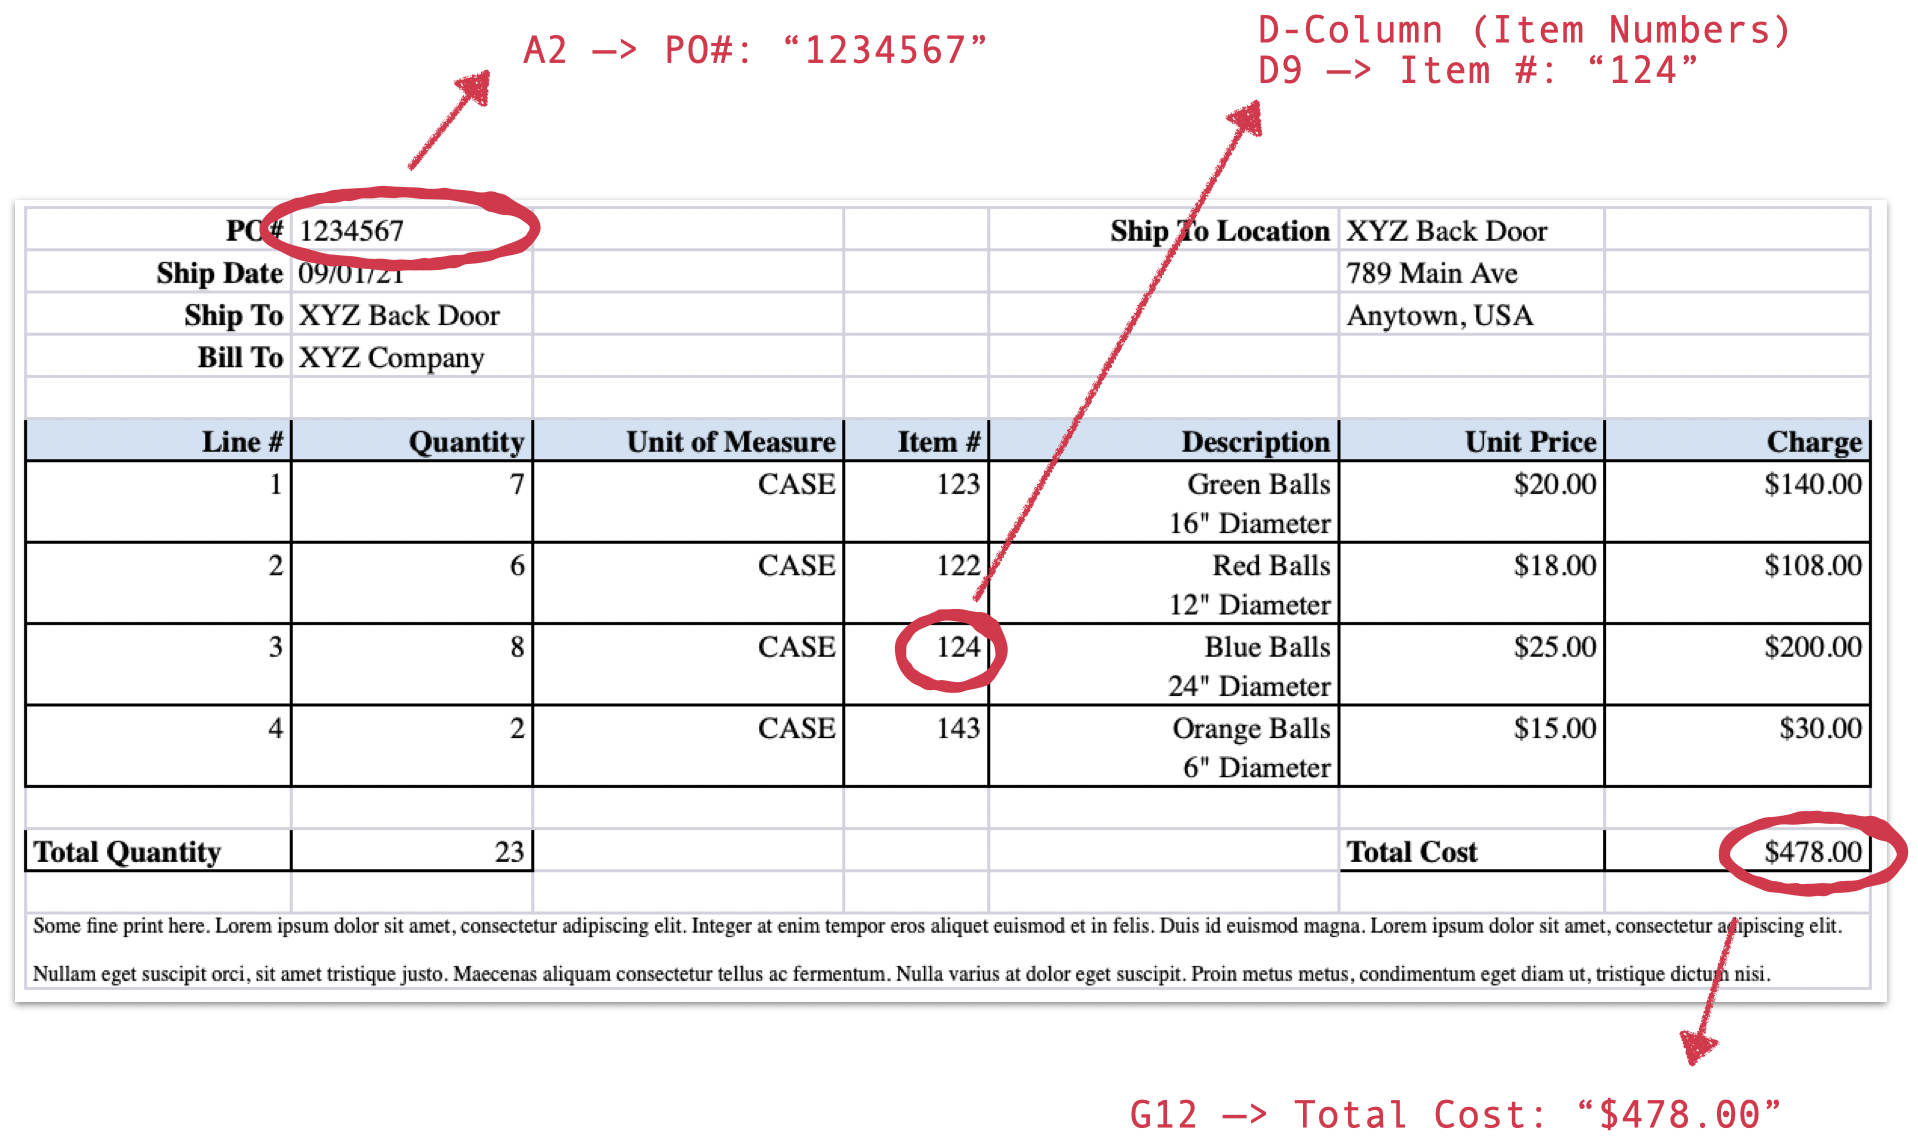
\includegraphics[width=\columnwidth]{RulesBasedApproach.png}}
\caption{We can programmatically find values in spreadsheets using positions and rules.}
\label{figRulesBasedApproach}
\end{figure}

A document like that in ``Fig.~\ref{figRulesBasedApproach}'' has values stored in specific cells within the document. If we know where to look, we can tell a computer program to extract that value and store it for us. For example, in our figure, we can see that cell A2 contains the value for our purchase order number, the D column (in cells 7-10) has item numbers, and G12 has the total cost. We can map these locations to variables where we want to store this information.

\subsection{Optical Character Recognition}
Optical Character Recognition, more commonly known as OCR, is a technique that results in converting images and files into machine-readable data (information in a form that a computer can process). The OCR technology reviews images for fonts and shapes, matching information with text that can be reviewed and stored.

While providing actionable information from different types of digital files, there are still many challenges with OCR. Images and pages may be received with incorrect orientation or skewed at an angle (imagine the paper is fed crookedly into a fax or scanner, or a picture taken with a phone that is not perfectly aligned). There may be noise or distortion on the page, or handwriting and other marks obscuring the printed text. If background colors or images are present, these can also impact the technology's ability to get a clear read on the information.

Some of these challenges can be overcome through the use of preprocessing. Pages can be scaled and adjusted to be the correct orientation. Filters can be applied to clean up noise. Newer iterations of OCR technologies also apply machine learning (ML) that can be used to better identify text characters when the image is unclear.

\begin{figure}[ht]
\centerline{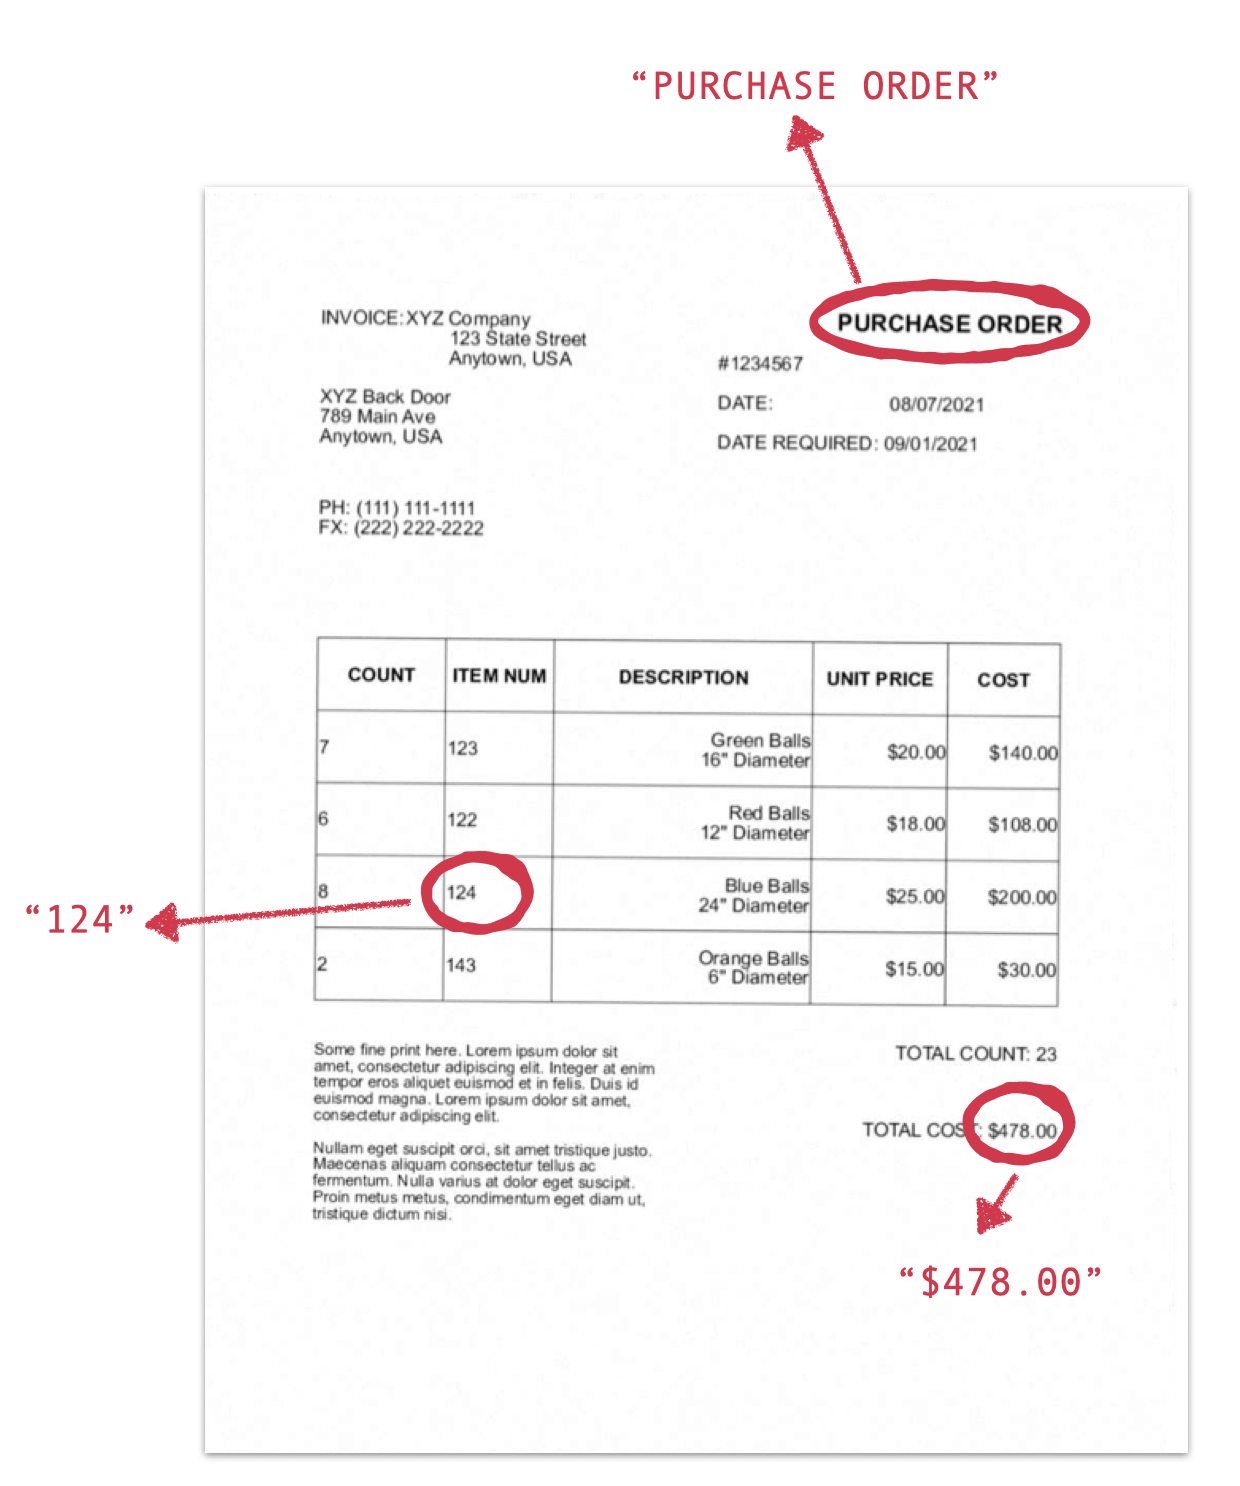
\includegraphics[width=\columnwidth]{RulesBasedOCR.png}}
\caption{Using OCR, we can translate the image into text, then we can programmatically find values for that text using positions and rules.}
\label{figRulesBasedOCR}
\end{figure}

Introducing OCR to the process of receiving files from customers gives us a digital version of the data. Rather than an employee typing the information character-for-character, output from an OCR engine provides the employee with data that can be copy-pasted with minor corrections. Combining OCR with the rules-based approach, we can gather data from an image programmatically (see ``Fig.~\ref{figRulesBasedOCR}'').  While small, this technique introduces some new efficiencies that we can leverage in an improved data processing flow.

\section{Processing Data} \label{sectionProcessingData}

Let's say we run a ball factory that produces balls of different colors and sizes. We receive orders from our customers in many ways. One of our customers submits orders using a templated spreadsheet generated from their internal system. Another customer faxes their (different) templated order along, which is then received digitally as a scanned image. Yet another sends an email message containing the information for their order. With more customers, there can be a wide variety of ways that orders are submitted!

Enforcing a specific business process could standardize the format and methods that customers use to place orders. We then might build an uncomplicated process to ingest orders using simple scripts and rules. Creating macros in our spreadsheets to process the information could also make it easy to enter into our ordering system.

\begin{figure}[ht]
\centerline{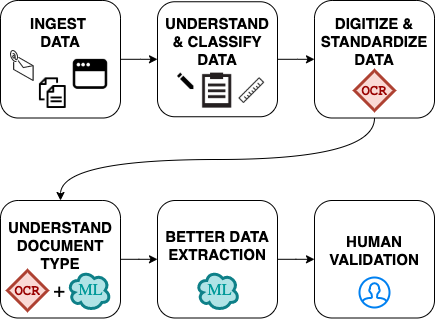
\includegraphics[width=\columnwidth]{HighLevelFlow.png}}
\caption{Document flow in a generic business process for extracting data from different inputs.}
\label{figHighLevelFlow}
\end{figure}

Not all companies will be able to expect a standard input on all customers; instead, they must consider how to handle the different types of documents by creating a business flow like the one in ``Fig.~\ref{figHighLevelFlow}''. The features in this general business flow are detailed below.

\subsection{Ingest Data}
The first step in our flow involves ingesting data. This means that we are receiving it somehow. The intake step may be an employee receiving a spreadsheet or a request written in the body of an email.

Some companies have different ingestion methods that allow for integrated flow to their ordering system, like having users place orders by logging into a website and entering their orders directly; with an integrated system, this order would then feed directly into the company's ERP. As our initially defined ideal scenario, integrated systems allow for little human error once the order has been entered by the customer. New businesses may have this option to directly integrate, but those that have been around longer may have customers that are accustomed to a certain method or may submit large volumes of data that make manual entry into a web application difficult.

To continue in our journey through this business process, we'll assume that we are ingesting documents that come in various types and formats and are not part of an integrated system. We will assume that our customer orders for our ball factory are entered manually.

\subsection{Understand \& Classify Data}
Since we are receiving orders in several file types (spreadsheet, pdf, email message, etc) that could be handled in different ways, we must find a method for understanding and classifying the data into one of three primary categories: Structured Data, Semi-Structured Data, and Unstructured Data. Once we have organized our documents into these groups, we can take the appropriate next action.

\subsubsection{Structured Data}
Often in the format of comma-separated values (CSV) and spreadsheets, structured data is formatted in a consistent template. The file contains tables with values in predictable positions. These documents could also be pdfs or other file types; the common thread is that the information is in the same layout for every document received.

Because of its predictability, this type of data can be gathered through simple data extraction scripts or template-based OCR. Rule-based approaches work well because we always know where to expect information that can be linked to a key-value pair (in the form of ``key: value'' like ``date: 8/14/2021'' or ``PO: 1234567'' where ``date'' and ``PO'' are keys).

\begin{figure}[ht]
\centerline{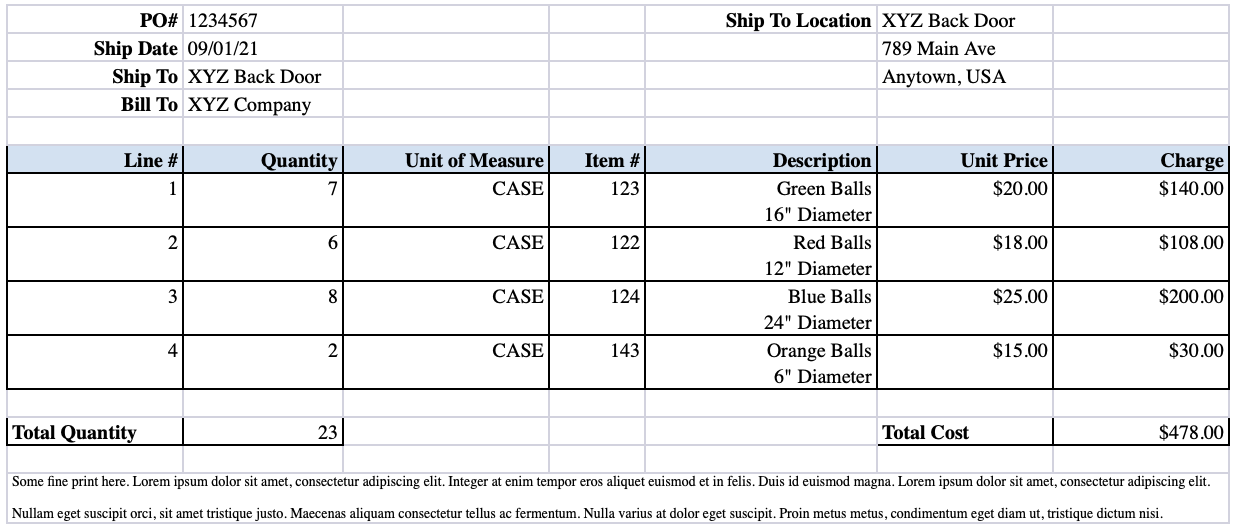
\includegraphics[width=\columnwidth]{Spreadsheet1.png}}
\caption{A templated spreadsheet for a purchase order.}
\label{figSpreadsheet1}
\end{figure}

Using our ball factory example, the spreadsheet in ``Fig.~\ref{figSpreadsheet1}'' could be an example of a structured document, if all spreadsheets received follow the same layout template. This structured data allows for scripts to be written that can map information by using the expected position of a value or with regular expressions to collect the value from the file. We've proven a sample of this in the simple Python code in Appendix \ref{appendixOrderOne} (for related unit tests, see Appendix \ref{appendixOrderOneTests}).

\begin{figure}[ht]
\centerline{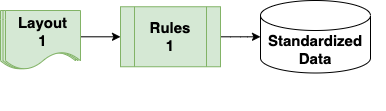
\includegraphics[width=\columnwidth]{RulesFlow1.png}}
\caption{All documents that match ``Layout 1'' can be passed through the same set of rules, ``Rules 1,'' extracting the values for each key piece of data in the document and storing in a standardized format.}
\label{figRulesFlow1}
\end{figure}

In ``Fig.~\ref{figRulesFlow1}'' we can imagine a straightforward set of rules that determines where information exists if all documents follow the same layout. When data is structured, we have a predictable place to look for the values we need, and gathering information in an automated method can be quite simple.

\begin{figure}[ht]
\centerline{
    \shadowbox{
        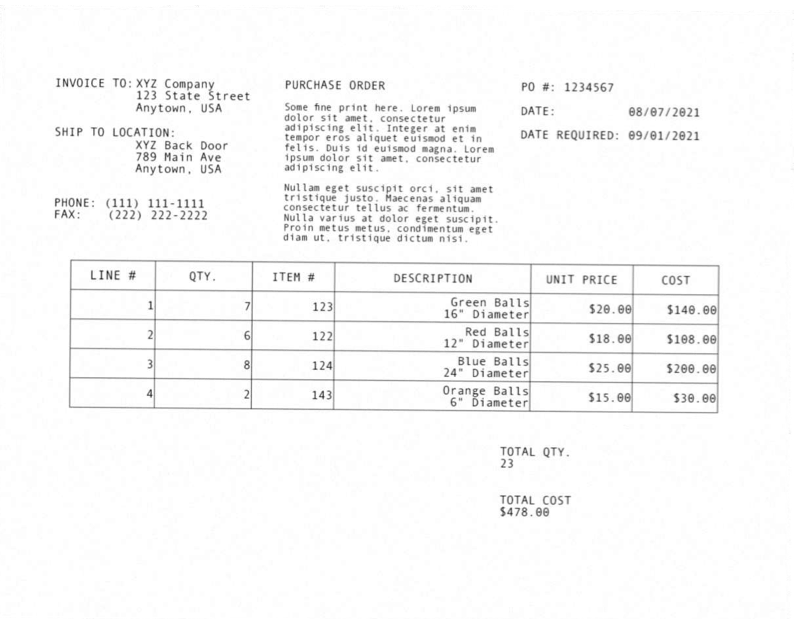
\includegraphics[width=200pt]{ORDER_1_scanned.png}
    }
}
\caption{A templated scanned image for a purchase order.}
\label{figScanned1}
\end{figure}

Similarly, we might receive a scanned image of a purchase order that equally follows a template (like that in ``Fig.~\ref{figScanned1}''), but must be read using OCR. Processing the file through a basic OCR reader could provide us with a data structure (see a small snippet of the type of data an OCR engine can produce in Appendix \ref{appendixOrderOneJSON}, which includes the word text and its position on the document), which can then be organized through additional scripts, though a bit more cumbersome to handle. Assuming all scanned images received are provided in this same layout, we can still treat the documents received as structured data.

\subsubsection{Semi-Structured Data}
If the same layout template of the structured data isn't followed, the changes or variations require new rules. New designs, layouts, or columns in a table of details might be a result of different regulations for a region requiring additional table columns in a purchase order, or larger customers using different systems that generate the files being provided.

\begin{figure}[ht]
\centerline{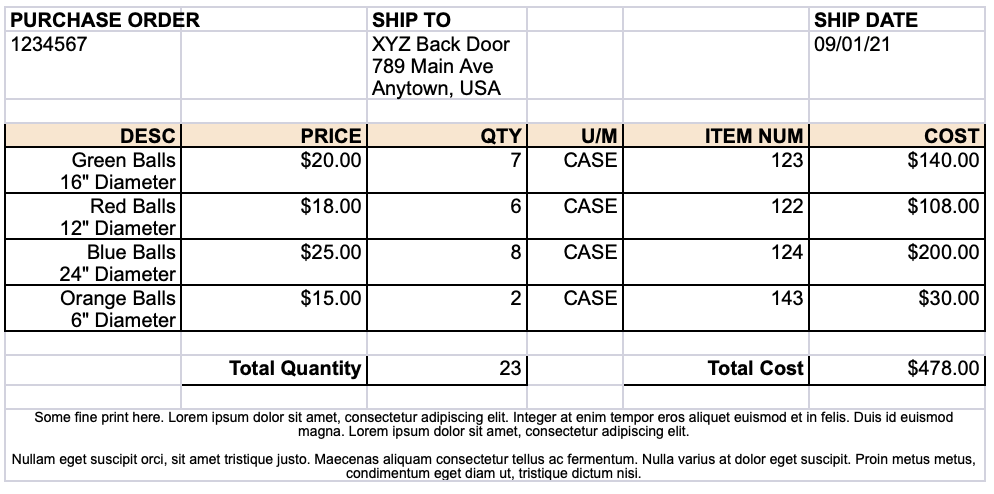
\includegraphics[width=\columnwidth]{Spreadsheet2.png}}
\caption{A templated spreadsheet for a purchase order containing similar information to ``Fig.~\ref{figSpreadsheet1}'', but with a different layout.}
\label{figSpreadsheet2}
\end{figure}

\begin{figure}[ht]
    \centerline{
    \shadowbox{
        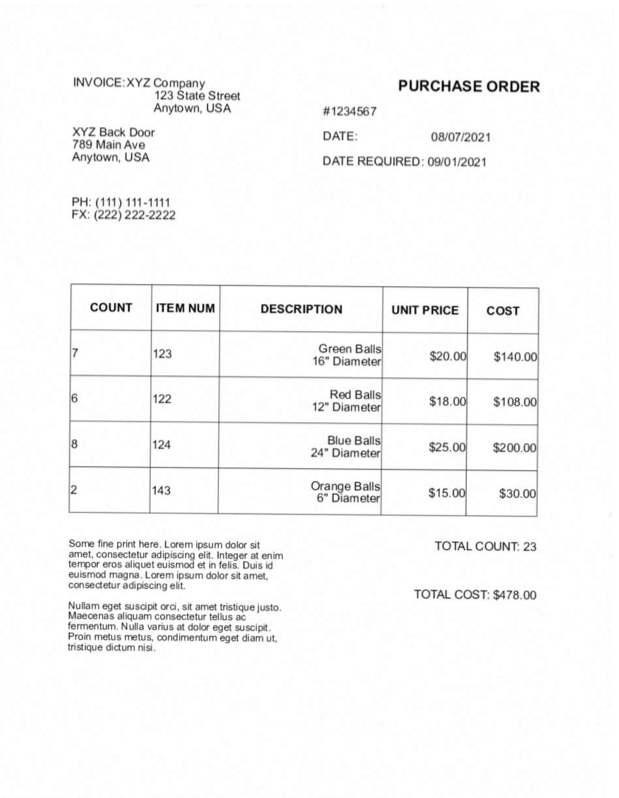
\includegraphics[width=160pt]{ORDER_2_scanned.png}
    }
}
\caption{A templated scanned image for a purchase order containing similar information to ``Fig.~\ref{figScanned1}'', but with a different layout.}
\label{figScanned2}
\end{figure}

Documents that contain the same type of information but in different designs and layouts fall into the category of semi-structured data. The keys in key-value pairs are the same across all documents, but the position on the page might vary, as seen in ``Fig.~\ref{figSpreadsheet2}''. Similarly, we might see scanned images like ``Fig.~\ref{figScanned2}'' with varied layouts.

\begin{figure}[ht]
\centerline{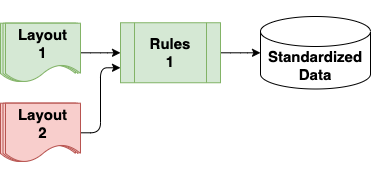
\includegraphics[width=\columnwidth]{RulesFlow2a.png}}
\caption{Documents with ``Layout 1'' applied to ``Rules 1'' will extract values with good accuracy, but documents with ``Layout 2'' applied to the same rules will extract values with low accuracy.}
\label{figRulesFlow2a}
\end{figure}

In this case, our rule-based approach gives us good accuracy for a document with one layout (ex: ``Layout 1''), but low accuracy for a document with another layout (ex: ``Layout 2''), like in ``Fig.~\ref{figRulesFlow2a}''. Appendix \ref{appendixOrderTwo} provides additional code that can be applied to the same methods used in Appendix \ref{appendixOrderOne} that will work for the spreadsheet in ``Fig.~\ref{figSpreadsheet2}'', providing an example of creating rules for each unique layout.

\begin{figure}[ht]
\centerline{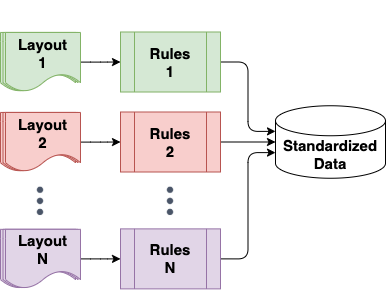
\includegraphics[width=\columnwidth]{RulesFlowN.png}}
\caption{For a large number of layouts, rule and template management becomes a job in itself and does not scale well.}
\label{figRulesFlow3}
\end{figure}

Writing a unique rule for each type is manageable when there are only a few variations in the layout templates. This approach of creating rules for every layout variation will have difficulty scaling for large volumes of semi-structured data (see ``Fig.~\ref{figRulesFlow3}''). Companies will have to devise a template creation and management process, adding and adjusting scripts and rules with each change and new layout.

Introducing artificial intelligence (AI) for growing volumes of semi-structured data can make it easier to scale at this stage of document classification and data extraction, avoiding template management. The field of AI combines computer science and hearty datasets to automate problem-solving \cite{ibm:ai}. Machine learning (a specific form of AI) uses models to automatically detect desired information from input documents. Machine learning (ML) applies algorithms to ``learn'' and improves accuracy in its program by receiving more samples to train on and improve its models. Vihar Kurama suggests the use of several pre-trained ML models (FastRCNN, Attention OCR, and Graph Convolution) for a hybrid solution of both rules-based data extraction and ML when working with semi-structured data such as our examples \cite{kurama2021a}.

Important to note is that the reliance on automated extraction should always be kept in check by a regular human review of metrics, accuracy, and confidence scores. Thankfully the processing of more samples through a machine learning model results in higher accuracy of the data retrieved.

\subsubsection{Unstructured Data}
The final classification for inputs received is unstructured data. This document type has no key-value pairs, may contain handwritten text, is free-flowing, and lacks consistency. Likely there are no tables (or the tables lack column headers) or a prescriptive way to automate the identification of which values to assign to which purposes. The message in ``Fig.~\ref{figUnstructuredEmailExample}'' is an example of unstructured information.

\begin{figure}[ht]
\centerline{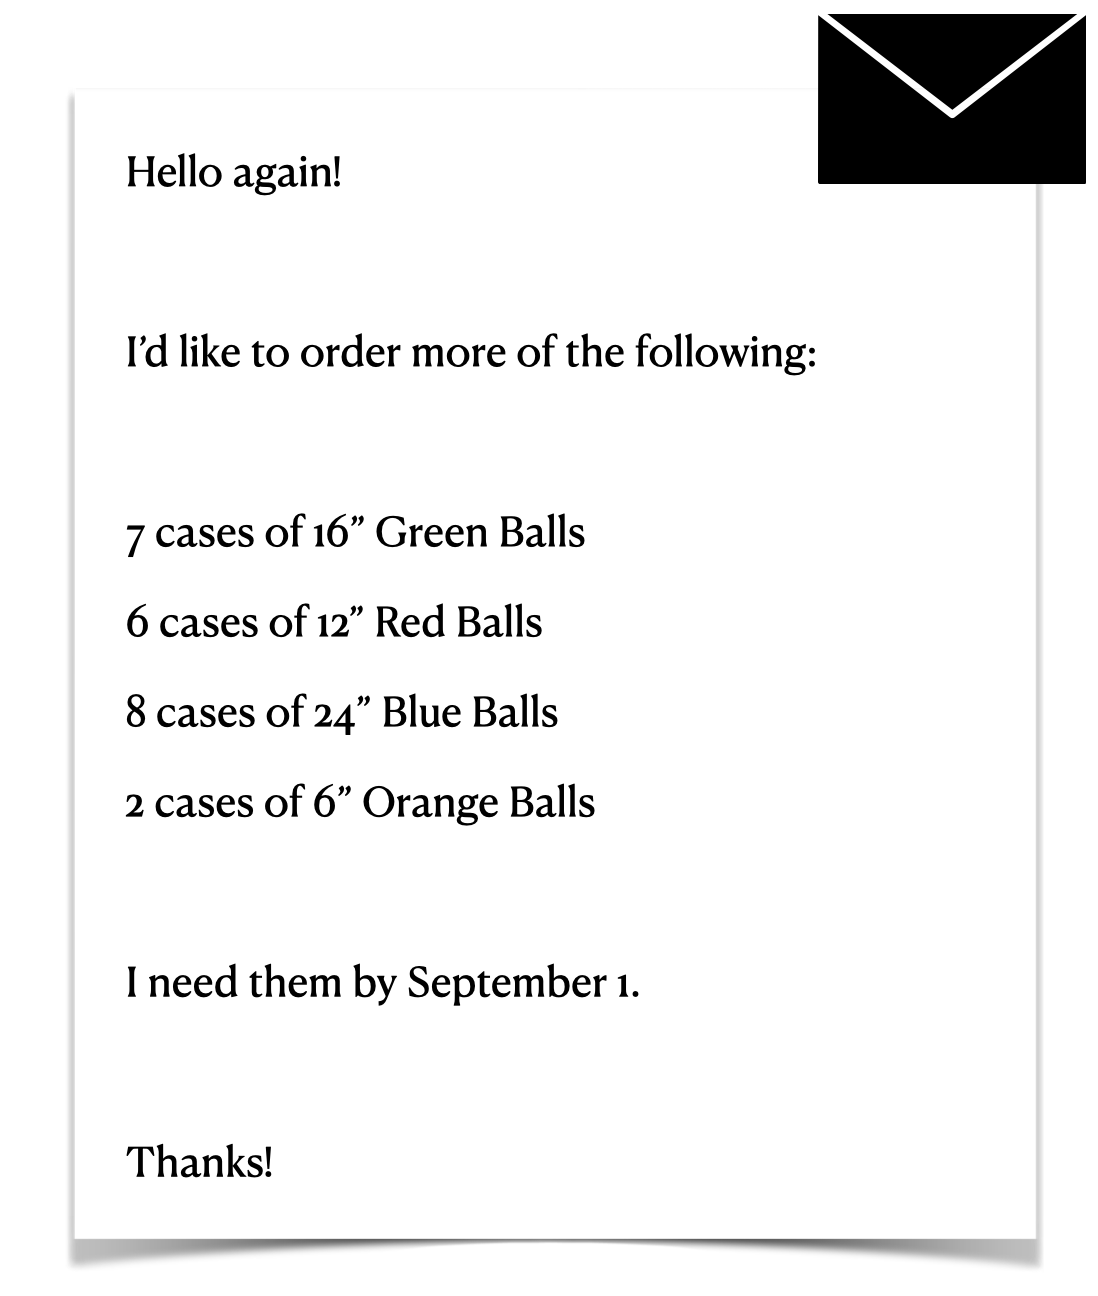
\includegraphics[width=150pt]{UnstructuredEmailExample.png}}
\caption{Messages like those received in emails are easy to understand from a human, but need to be translated to something a computer can understand using natural language processing (NLP).}
\label{figUnstructuredEmailExample}
\end{figure}

Scripts and ML are not enough to understand and classify this data. Instead, we may need to consider other techniques, such as natural language processing (NLP). Another branch of artificial intelligence, NLP provides computers with the ability to understand and translate the human language text of a document into something the machine can make decisions from \cite{ibm:nlp}.

\subsection{Digitize \& Standardize Data}
With the process of understanding and classifying our data as structured, semi-structured, or unstructured, we now have some digital information that we can put to use. Our first pass at the documents might not have been deep enough to understand the document type; our business process may be more efficient at this point to gather just enough information to determine where to feed the document. This may mean that we're capturing a page header, footer, or image with specific information to determine what type of document we're working with. 

\begin{figure}[ht]
\centerline{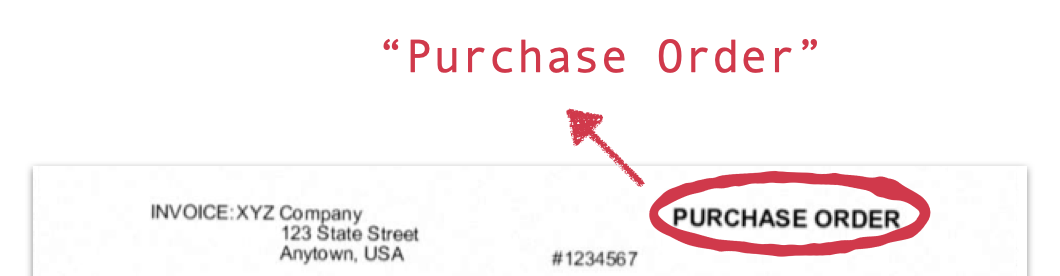
\includegraphics[width=\columnwidth]{DocumentHeader.png}}
\caption{Capturing information from the document header may help us categorize the document by type.}
\label{figDocumentHeader}
\end{figure}

\subsection{Understand Document Types}
With the standardized data from the previous step, we can determine if the document is an invoice, a purchase order, an application form, and so on. Documents that contain a ``purchase order'' header like in ``Fig.~\ref{figDocumentHeader}'' would get routed to the process for the ordering system, those with invoice headers might be sent to the Accounts Payable team, and application forms could be routed to the appropriate department, etc.

As a human, understanding the document types only takes a glance. If we consider automating this step for our pipeline, we need enough information to make the decision. If our data is structured, a rules-based system makes this very easy. Semi-structured and unstructured data can make this more difficult, especially if many document types are ingested into the same system. 

Depending on the complexity of the business process involved, we may consider introducing machine learning or natural language processing in this step. Or, we improve our ingestion step to separate document types by directing users to submit different types of documents to a specific email address, shared folder, web portal, etc. for each category we are receiving inputs for. The latter option may have some friction at the beginning but could be a very simple condition to overcome with a little customer training.

\subsection{Better Data Extraction}
Once we know our document type (invoice vs. purchase order, etc.) we can now apply more specific data extraction methods. This may be more heavily focused on machine learning models if the documents are semi-structured or natural language processing if they are unstructured.

\begin{figure}[ht]
\centerline{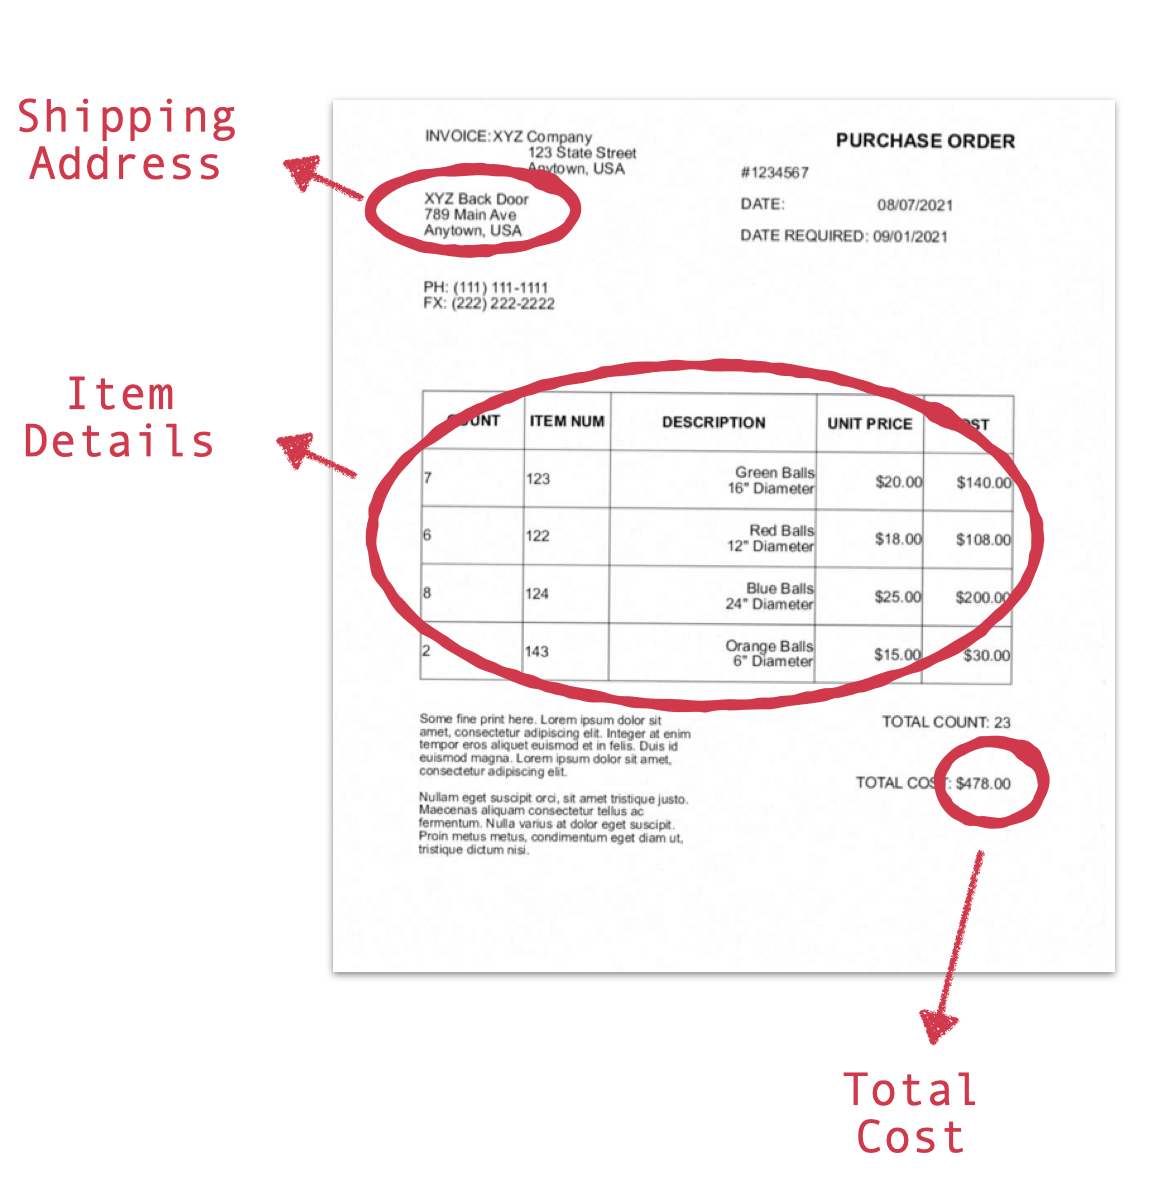
\includegraphics[width=\columnwidth]{BetterDataExtraction.png}}
\caption{Knowing our document type, we can do better data extraction. If our document type is a purchase order, we may know to extract the shipping address, item details, and total cost.}
\label{figBetterDataExtraction}
\end{figure}

Because we'll assume that our data is semi-structured for our ball factory, this stage is a good placement for intelligent OCR, that is, OCR that involves ML or some form of AI. Model-based OCR engines can improve the process of digitizing the documents at scale while continuing to reduce errors with every training.

\subsection{Human \& Automated Validation}
Nearing the end of our process flow, we've now reached the point where our data has been ingested and completely digitized into a standardized format. While it's true that with machine learning we may need fewer human checks as we train with more samples, a certain level of human-in-the-loop is necessary (and a good idea) when automating document handling. Confirming accurate information has been gathered from the ingested documents is vital for clean data and correct orders being created.

Thankfully, the continuous feed of more samples over time improves the ML model and builds confidence in the process. Regardless, there should always be a human check to verify incoming information.

Beyond the human check, we can also add automatic validation by cross-referencing the data we've gathered against information in our system(s). Do the item numbers and customer numbers found in the ingested document exist in our ERP system? Are the items in the order out of stock? If using machine learning or OCR, we can also flag low-confidence scores from the data extraction (rated by the OCR engine for how accurate it judges the results to be) for human review.

\section{Single Pipeline} \label{sectionSinglePipeline}
All of this has helped us understand the problem and an approach to handling documents. We have an idea of which types of tools might be useful and each particular step, but now we must understand how to string it all together into a single, cohesive pipeline, since finding a single solution is our goal!

A business process might begin as a simple macro or script, improving the time and effort needed for small tasks. From there, the process may see continued improvements through IT or business solutions. At some point, additional automation can be considered to raise the bar to another level: robotic process automation.

\subsection{Robotic Process Automation}
Robotic process automation, more commonly referred to as RPA, is the method of automating repetitive, often administrative, tasks. Generally speaking, virtual workers created for RPA will take advantage of a user interface on a screen, much like a human worker would do. These digital assistants will capture data and manipulate applications based on programmed decision-making. Similar to writing a programming script, RPA bots are made to mimic the same steps a human would do in particularly repetitive tasks, freeing up the human workers to focus on more valuable tasks.

While a powerful tool, the category of RPA is still relatively new in the technology field. In a survey of 100 document automation leaders by the Association of Intelligent Information Management, 18\% of the respondents use RPA and 12\% weren't sure of what RPA was. RPA with advanced capture has a place in the plans of 25\% of the respondents, but 42\% don't plan to make use of RPA. \cite{hollander2019survey}

Beyond standard RPA, where we simply automate the flow itself, we can level up our process some more by using intelligent RPA, which leverages forms of artificial intelligence, as we've already discussed, for document handling.

\begin{figure}[ht]
\centerline{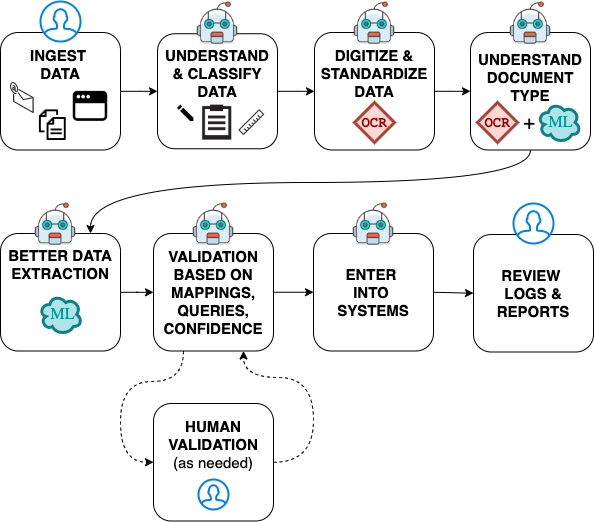
\includegraphics[width=\columnwidth]{BotFlow.png}}
\caption{Document Flow in a Business Process with RPA Bot and Human Worker ownership for each step.}
\label{figBotFlow}
\end{figure}

The flow in ``Fig.~\ref{figBotFlow}'' is similar to the business process we began with from ``Fig.~\ref{figHighLevelFlow}.'' However, we can see that with the use of RPA, it is possible to assign many of previous stages to a virtual worker; a human does not need to move the order document from one stage to the next. With the rules and AI in place, our digital assistant can not only ingest the data, but also classify, organize by type, standardize the data, validate it by cross-checking against existing table mappings (and alerting a human employee if further inspection is needed), but then also enter the data into the appropriate system (perhaps an ERP). Legacy systems may have no convenient integrations; RPA can interact with the user interface just like a human employee would, faster and with the cost-saving accuracy that a business requires.

This intelligent enhancement to a previously cumbersome and very manual flow frees up the human employees to turn their focus back to what matters: the value of customer relationships and understanding their needs to grow sales.

\subsection{Case Study: PepsiCo}
PepsiCo faced the challenge of a document processing flow that was slow, prone to errors, and very manual. When they applied a single process flow and involved the ABBYY FlexiCapture solution to their documents, they found that they had lower error rates, reduced processing times, and their Accounts Payable staff were able to work much more efficiently \cite{pepsico}.

PepsiCo's new flow is as follows:
\begin{enumerate}
\item Paper invoices (in any of 5 languages) are scanned locally
\item Scanned invoices are...
    \begin{enumerate}
        \item sent to the POWER Project
        \item identified with the correct entity
        \item recognized by FlexiCapture
    \end{enumerate}
\item New digital documents and data are sent to verification stations
\item Data is verified
\item Data is forwarded to PepsiCo's Image Vision for approval
\item Data is exported in XML
\item Data is processed in PepsiCo's SAP ERP solution
\end{enumerate}

``FlexiCapture's accuracy is also proving stable under a heavy workload. In its first three months the POWER Project solution has processed two thousand batches, over 21,000 documents and nearly 40,000 pages without issues – in a mix of five languages.'' \cite{pepsico}

In a review done by PricewaterhouseCoopers (PwC), ABBYY FlexiCapture was rated best in class in data validation and data classification, as well as data extraction in both structured and semi-structured documents. It also ranked well for multi-lingual capabilities, and the ability to read barcodes and tables. Google Tesseract and Microsoft's Modi ranked better for screenscraping in desktop, web, and documents. PwC goes on to note that ``the integration of the ABBYY OCR engine not only enhances automation for rules-driven processes, but also adds the flavour of NLP and widens the scope of automation.'' \cite{pwc2018robotic}

This single pipeline solution has proven that it can scale and do it well! Powerful tools that fit the specific process need, like ABBYY FlexiCapture, combined with the power of automation, enabled PepsiCo to not only improve the intake process for documents at one location but to create a solution that accurately processed the information and can be scaled across the entire enterprise.

\subsection{Case Study: Sysco}
With a similar need and desire to improve the business processes, Sysco set out to also improve the accuracy and efficiency of many tasks across the company. By creating a team focused on RPA solutions, Sysco sought to create a new culture around automation enterprise-wide.

The Sysco RPA team has provided more than 200,000 hours of productivity given back to the business and has handled over 5.1 million transactions over the first 3.5 years of the team's existence. Over 150 automations have been created and span across almost all business units. Their expansion looks to include specialty companies outside of the United States and includes a growing pipeline of over 200 business processes that are automation candidates. \cite{bpcafe2021sysco:slides}

With at least one automation that involved OCR tools used to parse digital faxes, the Sysco team explored several other solutions varying from simple rules-based automations to more complicated and impactful processes \cite{bpcafe2021sysco}. Interestingly, this team not only standardizes and automates processes for other business units but also created a standardized business process and development pod structure to improve their efficiency and accuracy in determining which automations to create next and in the bot construction process itself.

\subsection{General Application}
While the case studies presented above provide compelling narratives of the power of RPA in combination with OCR and AI, it may be difficult to understand where to begin. By identifying business cases that are repetitive and have a volume of effort that could be reduced through the use of scripts or automations, we have a place to start.

\begin{figure}[ht]
\centerline{
\includegraphics[width=\columnwidth]{USE CASE - 1 - STRUCTURED.png}}
\caption{Starting with an automated flow for only structured documents allows for full understanding of the process and gets employees familiar with using an RPA virtual assistant. Limiting the input to a single layout also eliminates needing to classify the data and determine the document type.}
\label{figUseCase1}
\end{figure}

Businesses may experience a temptation to view automation as an all-or-nothing scenario. By starting with a small section of automation first, like ``Fig.~\ref{figUseCase1},'' we can provide benefits quite quickly. Automating small steps in a process provides an opportunity to work out issues (not only bugs in the programming but also finding flaws or forgotten exceptions in the business process itself). When chosen correctly, automating one step in a business process can deliver a return on investment as soon as the feature is being adopted by users. This smaller section of process automation also helps us to understand nuances and challenges before we move on to more complicated stages.

\begin{figure}[ht]
\centerline{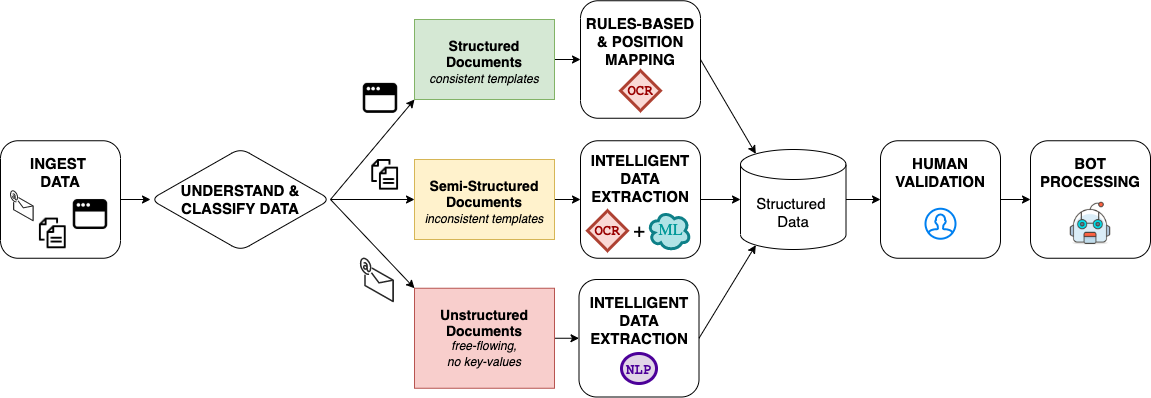
\includegraphics[width=\columnwidth]{USE CASE - 4 - ALL.png}}
\caption{By starting with one flow and adding in more entry points that lead to the same structured data, we can expand our automated process in an iterative way.}
\label{figUseCase4}
\end{figure}

By each iteration of our process flow, we can provide new input formats that are handled by different rules and technologies (``Fig.~\ref{figUseCase4}''). We can add handling for structured data that is received through our web application, semi-structured data received as files on a shared drive, and unstructured data captured in an email message. We can continue to expand for all data classifications while still leveraging the automated stages we built in the first round once the data is stored in a standardized format.

With many powerful solutions out there, advantages can be found in small steps first. Are employees typing in data from paper forms regularly? First, determine if the business process itself can change to an integrated solution. If it is not feasible to have the user change their input method within a reasonable timeframe, continue with the existing process and begin improving it by ensuring that those documents have been scanned into a system. Once digitally saved, run an OCR engine against the document, providing your employees with something they can at least copy-paste. Or, perhaps you already have the information in structured spreadsheets. Write a script that automatically captures the key-value pairs and table data, storing the information in a standardized format like a database. Once the process flow is working smoothly to the point of consistent and standardized information, consider adding some type of automated solution that can enter the data directly into the system, rather than an employee copying the information in.

By taking small, iterative steps, any company, large or small, can work its way into an automated flow. While some solutions like ABBYY FlexiCapture can provide top-of-the-line solutions, the cost may be prohibitive to some businesses. Start with the standard, rules-based methods, and enhance the areas that will still provide enough return-on-investment to justify the effort. The beautiful thing about the single-process pipeline idea is that more document types could be ingested over time, training the process with where to send each type. Some stages might continue to be human-handled, but there may be small improvements that allow the human to perform that step faster, like a dashboard that gives the employee a preview of the document. These types of process improvements might enable an employee to quickly glance and classify the information manually. Process improvement may save on the implementation of intelligent OCR or ML while still providing time-saving benefits.

\section{Solutions \& Considerations} \label{sectionCosts}
There are many tools out there and it can quickly become overwhelming to narrow them down. If you're entering into the field of RPA, you may choose a solution that is integrated into an existing RPA platform, like Blue Prism's Decipher or Automation Hero. Perhaps you work with spreadsheets and gravitate towards Altair's Monarch. Microsoft has an entire suite of options with the Microsoft Power Apps. And we can't forget the solutions that Amazon provides.

Each tool has its strengths and weaknesses, in addition to varying levels of cost. Understand the types of documents you'll be working with and determine your needs. If you've started with automating structured documents, and are ready to include other classifications that require intelligent sorting, consider which models and training might be necessary.

I've heard the phrases, ``the best exercise is the one you'll do,'' or ``the best camera is the one in your hand.'' This idea can apply here as well: the best tool to improve your process is whichever one you start using. One technology may not have huge advantages over another. Some options may be tightly coupled to their own branded integrations. Others might have a nicer user interface. Becoming paralyzed by the number of solutions available is a possibility; give your research period a time-box, then choose whichever option(s) best suit the business needs and the skills of your technical team.

\section{Conclusion}
Manual data entry is time-consuming and error-prone. The introduction of OCR (combined with ML) or NLP can result in fewer typos during data extraction and opens the door to the improved process flow. Beyond that, considering RPA within the business process can create further efficiencies, giving skilled employees time back to focus on more valuable tasks that have a higher impact on the company's profitability.

Many well-tested solutions are available, with pre-trained models ready to implement from the start, reducing the number of required samples to get a machine learning solution off the ground quickly. However, the strongest solutions can be cost-prohibitive. Not to be deterred, we can still provide improvements by automating smaller sections of the process flow or enhancing the human step (thus bypassing the need for intelligent automation) to make it simpler to perform.

While still a young category of technology, RPA provides further enhancements by not only stringing together the steps into a single process flow but also moving into working with legacy systems without the need to wait for modern integrations.

Depending on the business needs, more research can (and should) be done on which tools may provide the best solutions. A quick search on the web can provide appropriate overviews of the most popular tools. For example, Nanonets provides a list of pros and cons for the best OCR tools of 2021 \cite{prithiv2021best}. Depending on the needs and time available (for development and potential training of models) for each business case, the right tool for the job may change.

Iterating through development is key for a quick return on investment and limiting rework. Starting with rule-based solutions can provide a solution that is faster to deliver and provides insights into nuances and challenges within the process flow. Expanding into RPA in the next iteration builds confidence and trust in the automation, freeing up more time for human employees to focus on valuable tasks. Entering into intelligent RPA opens the floodgates to the types of documents that can be handled automatically, with human review.

The problem at hand is that data can be received in many formats; manually extracting that information can be tedious at best and riddled with errors at its worst. Is there a single-process solution that businesses can implement to improve this process? Each business process has some unique nuances that require specific solutions. Some very powerful options are out there that provide less training and setup. However, all companies can start with small solutions (even improving the business process itself!), then iterate and build on those solutions creating a robust, single-process built of many small steps.

\newpage
\bibliographystyle{unsrt}
\bibliography{bibliography}

\onecolumn
\appendices

\newpage
\section{Python Methods to Collect Data from a Spreadsheet} \label{appendixOrderOne}
    \subsection{spreadsheets/methods.py}
    \lstinputlisting[language=Python]{Scripts/spreadsheets/methods.py}

    \newpage
    \subsection{spreadsheets/excel\_order\_one.py}
    These mappings are specific to the spreadsheet represented in ``Fig.~\ref{figSpreadsheet1}''.
    \lstinputlisting[language=Python]{Scripts/spreadsheets/excel_order_one.py}

\newpage
\section{Unit Tests for Python Methods in Appendix \ref{appendixOrderOne}} \label{appendixOrderOneTests}
    \subsection{tests/test\_spreadsheets\_methods.py}
    \lstinputlisting[language=Python]{Scripts/tests/test_spreadsheets_methods.py}

    \newpage
    \subsection{tests/test\_excel\_order\_one.py}
    \lstinputlisting[language=Python]{Scripts/tests/test_excel_order_one.py}

\newpage
\section{Data Collected as JSON from a Scanned Image} \label{appendixOrderOneJSON}
A full sample of the JSON for the scanned image from Order 1 (``Fig.~\ref{figScanned1}''), generated by an OCR scanning tool (OCRSpace \cite{ocrspace}), can be found stored on GitHub: \url{https://github.com/amajor/research-in-cs-course-project/blob/main/Scripts/documents/OCRSpace\_Order1.json}

A full sample of the JSON for the scanned image from Order 2 (``Fig.~\ref{figScanned2}''), generated by an OCR scanning tool (OCRSpace \cite{ocrspace}), can be found stored on GitHub: \url{https://github.com/amajor/research-in-cs-course-project/blob/main/Scripts/documents/OCRSpace\_Order2.json}

Below is a very small sampling of some lines at the beginning of a JSON file (lines 1-40) containing the data recognized from the scanned image (``Fig.~\ref{figScanned1}''):
\lstinputlisting[language=json, linerange={1-40}]{Scripts/documents/OCRSpace_Order1.json}

% ====== Something in these lines of code causes references to be unable to render ====== %
% \newpage
% Below is a very small sampling of some lines at the end of a JSON file (lines 1484-1519) containing the data recognized from the scanned image (``Fig.~\ref{figScanned1}''):
% \lstinputlisting[language=json, linerange={1484-1519}]{Scripts/documents/OCRSpace_Order1.json}

\newpage
\section{Python Methods to Collect Data from a Spreadsheet} \label{appendixOrderTwo}
    \subsection{spreadsheets/excel\_order\_two.py}
    These mappings are specific to the spreadsheet represented in ``Fig.~\ref{figSpreadsheet2}''.
    \lstinputlisting[language=Python]{Scripts/spreadsheets/excel_order_two.py}

\newpage
\section{Unit Tests for Python Mappings for Spreadsheet Order Two} \label{appendixOrderTwoTests}
    \subsection{tests/test\_excel\_order\_two.py}
    \lstinputlisting[language=Python]{Scripts/tests/test_excel_order_two.py}

\end{document}
